\chapter{Scaling}\label{sec:scaling}

For spatial discretization implicit schemes are used. Hence, the calculation of
a derivative always involves communication amongst all processors in a line
along which a derivative is computed. From ad-hoc considerations it is not clear
which is the optimum two-dimensional domain-decomposition.  While for small
numbers of cores one would expect the network latency of an MPI call to
dominate, for larger numbers it is the number of processors involved in the call
that makes MPI calls expensive. Therefore, below a certain threshold, a 1D
decomposition is expected to be beneficial. Where this turnover takes place is
subject to many factors such as the CPU clock speed, network latency, MPI
implementation, number of grid points, etc.

We briefly introduce now definitions and notation used in the rest of this
section. We define $Q:=q_x\times q_y \times q_z$, the number of grid points, as
a measure of the size of the simulations and choose in the following to label
simulations by $Q$. To label the simulations, we use the common abbreviations
\begin{equation}
\kilo=2^{10};\qquad\mega=2^{20};\qquad\giga=2^{30}
\end{equation}
for readability. The memory necessary to save one 3D array in double precision
data format is $8\times Q~\mathrm{Byte}$.  The scaling of the code is discussed
in terms of speedup $S$ and efficiency $\eta$ defined as
\begin{equation}
 S:=\frac{T}{T_\mathrm{ref}}\qquad \eta = \frac{T}{NT_\mathrm{ref}} \times 100\%,
\end{equation}
where $T$ is the real time to run a particular case, $N$ the number of
processors and the subscript 'ref' indicates a reference value.

The code has been instrumented to measure the real time that is necessary to
perform one stage of the multi-stage Runge-Kutta time-stepping scheme.  This
corresponds essentially to the evaluation of the right-hand-side term of the
governing equations solved. The pre-processor flag \verb,-DUSE_PROFILE,
activates it and data is written into the log file \verb,dns.log,. The aim is to
remove the overhead time associated with I/O and initialization.

\section{Scaling on the cluster \texttt{jugene@fz-juelich.de}}

Performance of the DNS code has been measured for various geometries varying the
total number of grid points by two orders of magnitude. Many-core scaling
properties of the DNS code, version 5.6.6 on the
machine \texttt{jugene@fz-juelich.de} (site J{\"u}lich Supercomputing Center)
were investigated. All simulations have been run in SMP mode using 4 OpenMP
threads, reaching up to up to 8k MPI tasks distributed over 8k nodes (1 rack
contains 1k nodes), using 4 cores per node (i.e. 32k cores in total). Linear
scaling is observed for up to 4096 MPI tasks using about 6-8 \mega~grid points
per processor (domains of 24-32 \giga~grid points).  The maximum efficiency is
usually reached when simulations are carried out within one mid-plane. In this
case, a slightly super-linear scaling (with respect to the reference at 32
nodes) is observed for the standard domain sizes of up to 4 \giga~grid points.

\begin{table}[!ht]
\begin{centering}
\begin{tabular}{p{2cm} p{0.5cm} p{0.5cm} p{0.5cm} p{1.cm} }
\toprule
Name& $q_x$& $q_y$& $q_z$& $Q$\\
\midrule
\texttt{1024x0384}& 1024& 1024&  384& 384 \mega\\
\texttt{2048x0192}& 2048& 2048&  192& 768 \mega\\
\texttt{2048x1024}& 2048& 2048& 1024&   4 \giga\\
\texttt{3072x1536}& 3072& 3072& 1536&  12 \giga\\
\texttt{4096x1536}& 4096& 4096& 1536&  24 \giga\\
\texttt{4096x2048}& 4096& 4096& 2048&  32 \giga\\
\bottomrule \\
\end{tabular}\\
\caption{Geometry and labels of the 3D cases.}
\label{tab:sim_table}
\end{centering}
\end{table}

The code has been run for 2 iterations, i.e. 10 Runge-Kutta stages using the
fourth-order, five-stages algorithm, and the variance of measured times was
found to be of the order of 1\%.  The cases considered here are listed in
Table \ref{tab:sim_table}.

\subsection{Strong Scaling}\label{sec:domain_decomposition}

The total number of MPI tasks (nodes) available to a simulation are distributed
as $N = $\texttt{ims\_npro} = \texttt{ims\_npro\_k}
$\times$ \texttt{ims\_npro\_i} in the directions of $k$ ($z$) and $i$ ($x$). A
series of measurements has been carried out to determine the optimum
configuration for the six cases listed in table
\ref{tab:sim_table}. Scaling matrices are shown in Figures \ref{fig:matrices1}
and \ref{fig:matrices2} for the different cases.  In these matrices the number
of processors is constant along diagonals from the lower left to the upper
right. In every matrix, the diagonal for $N=1k$ MPI tasks is outlined by solid
borders. In each of these diagonals, the best and worst configurations are
marked by green, respectively red, color. In these matrices, the speed-up and
efficiency is for strong scaling, and always calculated with respect to the time
$T_\text{ref}$ for the lowest number of cores with the
lowest \texttt{ims\_npro\_i}. Efficiency $\eta$ and speed-up $S$ are calculated
as above. The shapes used in the simulations, that is, the relative connection
among mid-planes, is $1\times 1\times 1$, $2\times 1\times 1$, $2\times 2\times
1$, $2\times 2\times 2$, $4\times 2\times 2$, ordered from 1 mid-plane (512
nodes) to 16 mid-planes (8192 nodes).

\begin{figure}
\begin{centering}
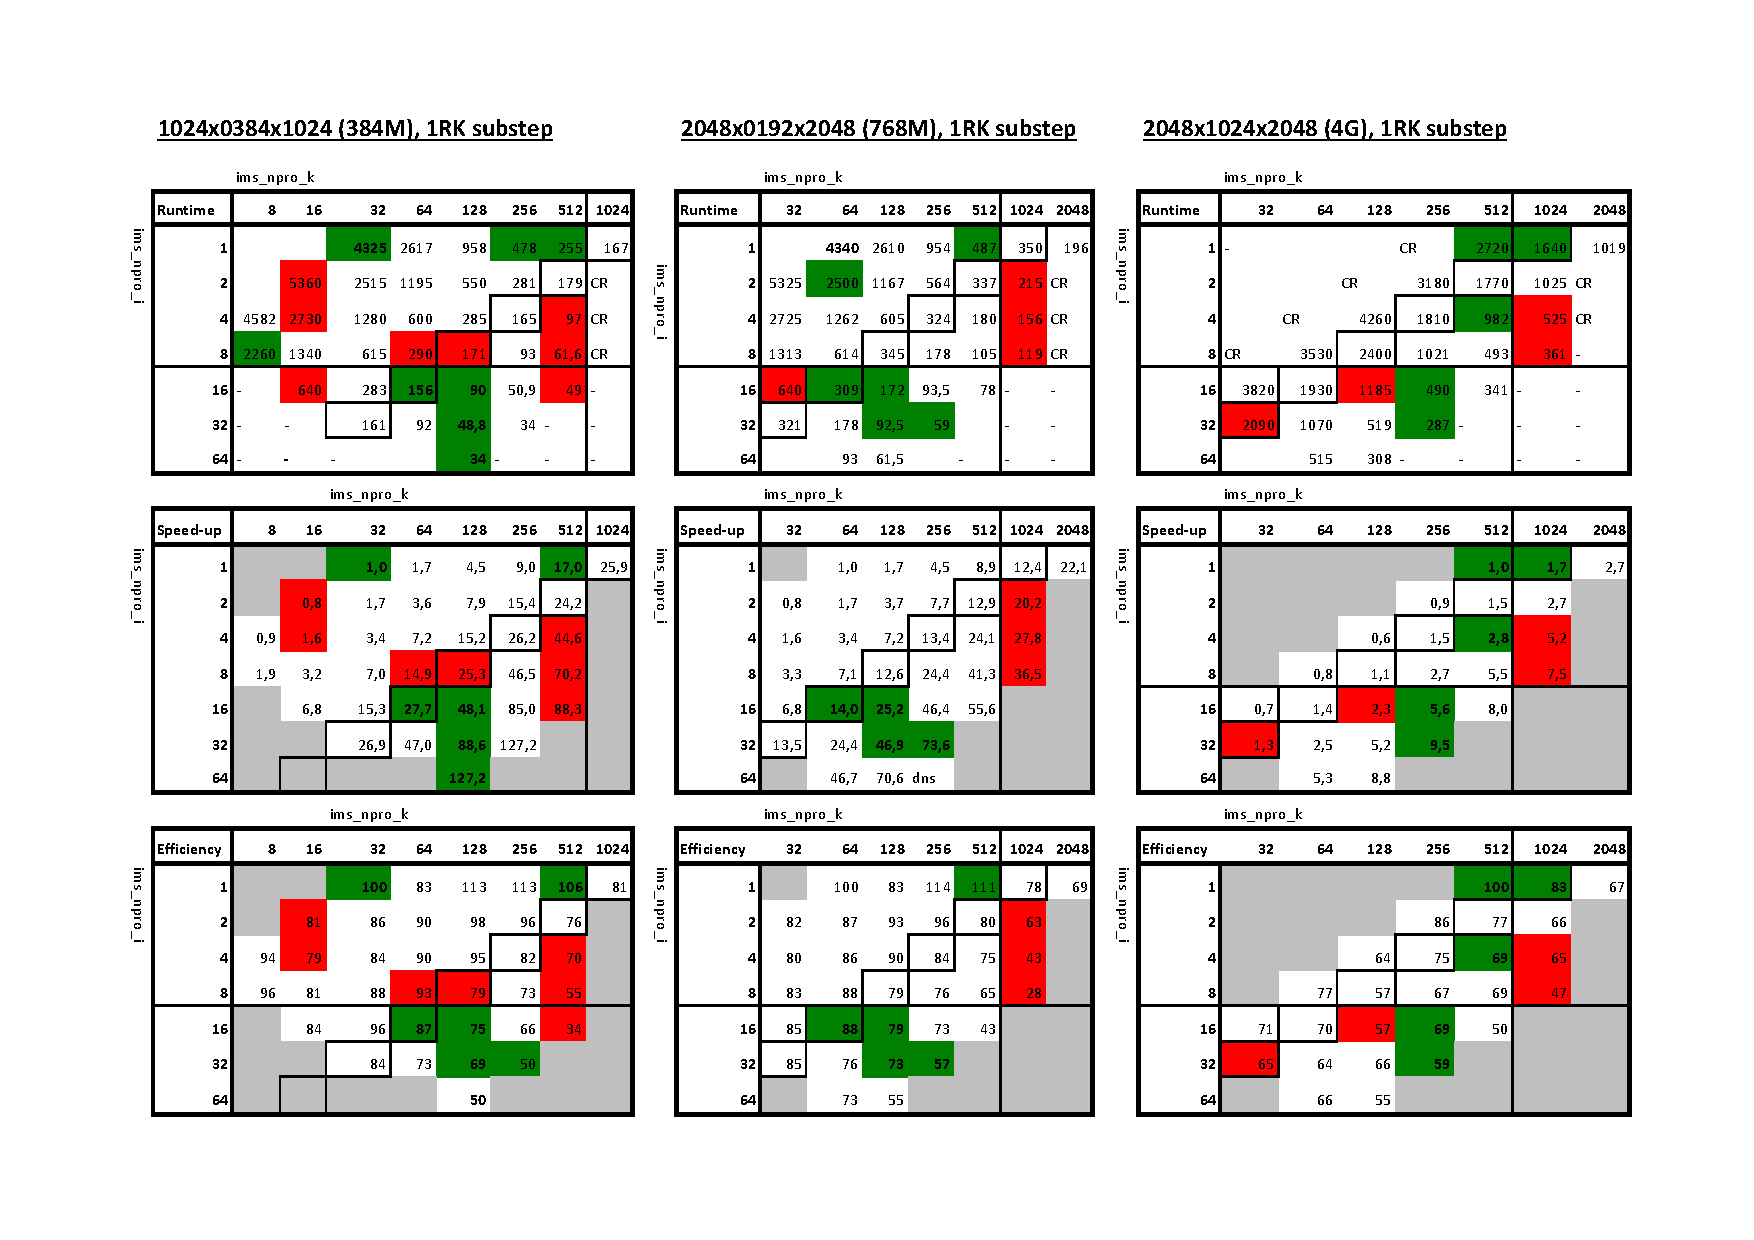
\includegraphics[height=0.9\textwidth,angle=90]{figs/matrices_1.pdf}
\caption{Matrices for scaling and 2D domain decomposition. Time is in hundredth
  of a second per single Runge-Kutta stage. In the time-matrices, simulations
  that crashed because of too little memory (above diagonals) and page problems
  (below diagonals) are marked by \texttt{CR}. If no measurement for a certain
  configuration was attempted, the cell is left empty. For speed-up and
  efficiency all configurations not available are marked gray.}
\label{fig:matrices1}
\end{centering}
\end{figure}

\begin{figure}
\begin{centering}
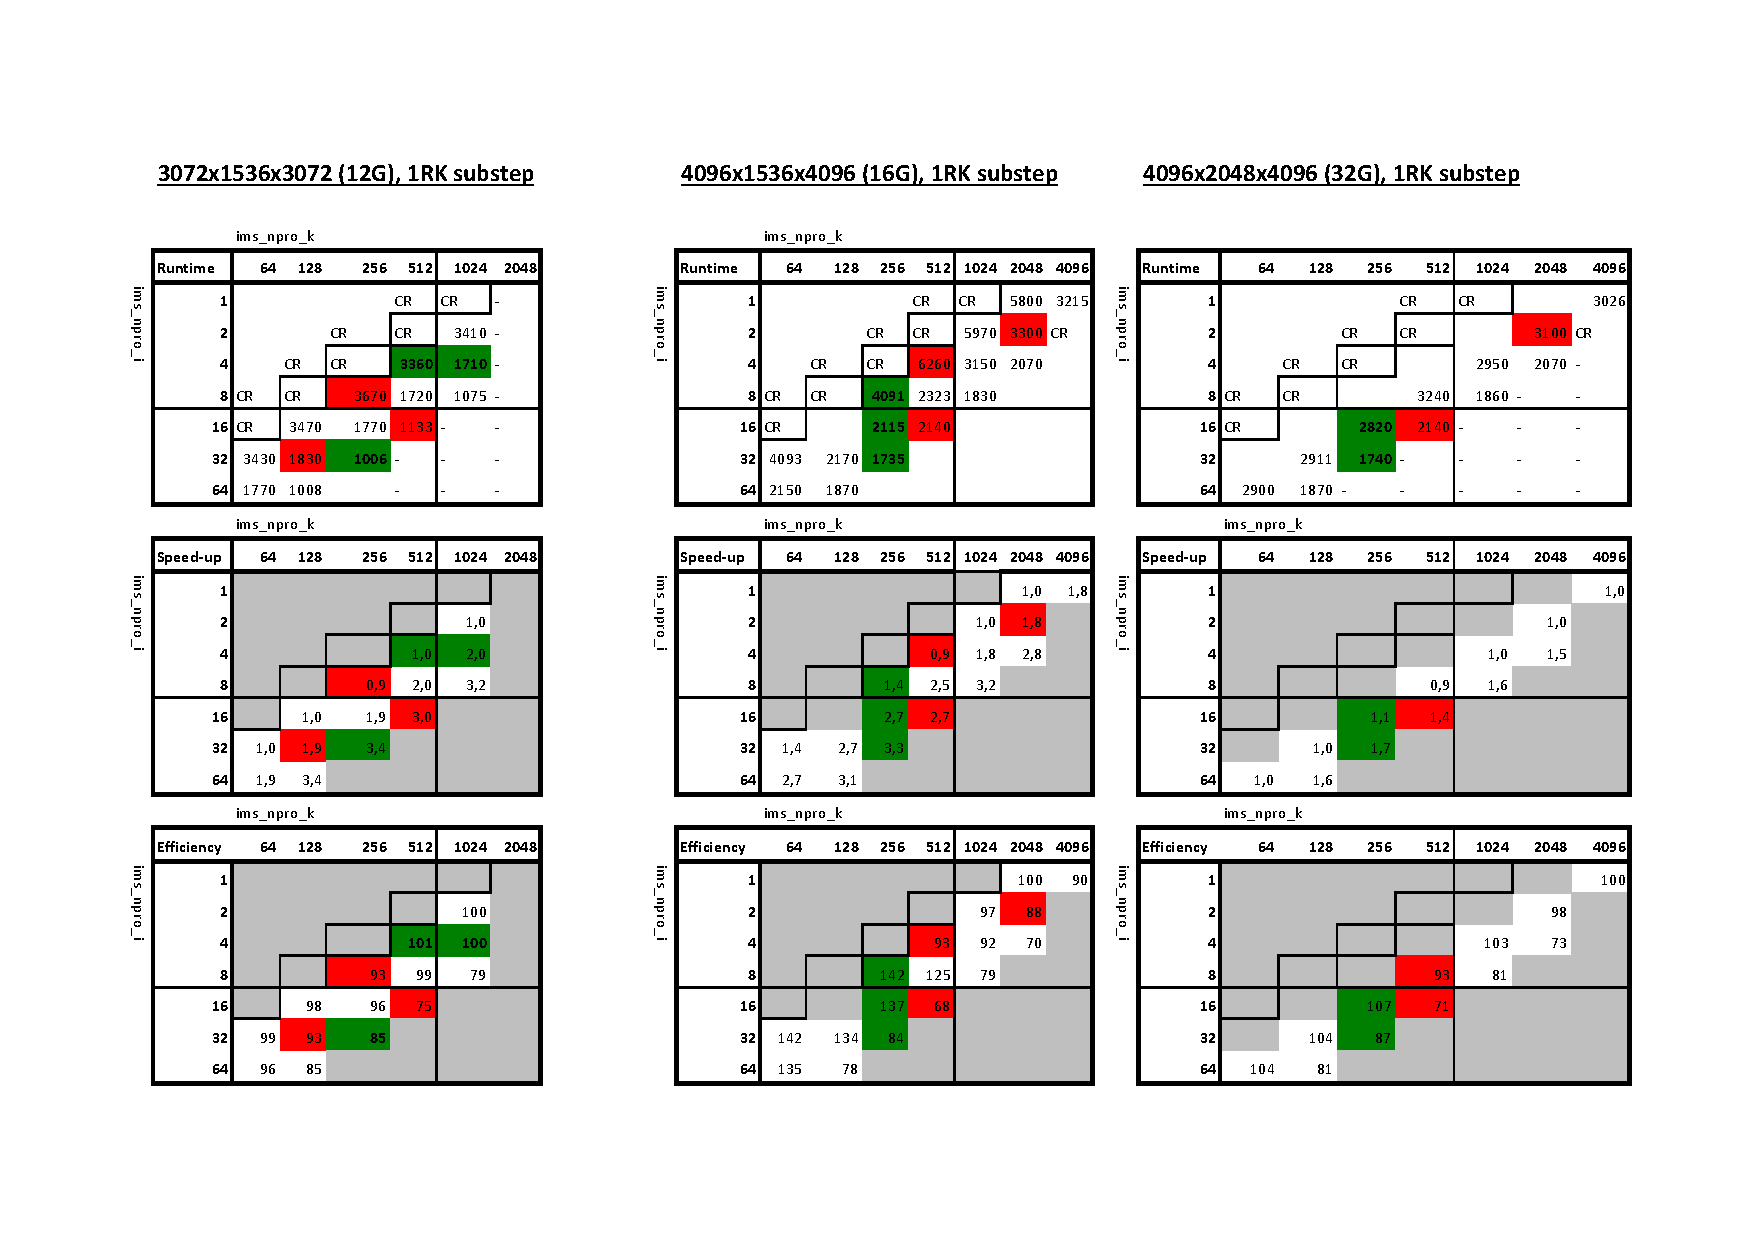
\includegraphics[height=0.9\textwidth,angle=90]{figs/matrices_2.pdf}
\caption{More cases. Same legend as in Figure~\ref{fig:matrices1}.}
\label{fig:matrices2}
\end{centering}
\end{figure}

\subsection{Scaling from 32 to 8192 nodes}

A strong scaling analysis over the entire range of nodes from 32 to 8192 is not
possible. Hence, we restrict ourselves to a scaling analysis where we consider
the number of grid points that is handled per processor and time unit. A
straightforward definition for a metric of performance $P$ is
\begin{equation}
  P:=\frac{Q}{N T} \;,
\end{equation}
the number of grid points processed per node and per time. $T$ is the time
needed by each of the cases to advance exactly the same amount of instructions
in the main algorithm, e.g. one stage of the Runge-Kutta scheme. $P$ is a metric
that makes performance comparable over \textit{almost} arbitrary problem sizes
and numbers of cores.

Note, that the caveat here is the operation count for the Fourier transforms
which goes as $q_i \log q_i$ and $q_i \approx Q^{1/3}$ if domains are expanded
by the same factor in each direction. Hence, for the overall operation count of
the Fourier transforms $\Sigma_\mathrm{FFT}$ we get
\begin{equation}
\frac{\Sigma_{\mathrm{FFT}}}{q_{i}^{2}}\propto 3 q_i \log q_i = Q^{1/3} \log
Q\Rightarrow \Sigma_\mathrm{FFT}\propto Q\log Q.
\end{equation}
For the range of $Q$ considered here, this effect is, however, small since the
super-linear contribution of $\Sigma_\mathrm{FFT}$ is only $\frac{\log 32\giga
}{\log 384\mega} \approx 1.2$ and the FFT accounts for a negligible part of the
computational time ($1\%-5$\% of the computational part, which is
$0.5$\%-$2.5$\% of the overall time).  The operation count of the rest of the
algorithms is linear.

Given $P$, one can compute a virtual efficiency and speed-up $\eta_v$ and $S_v$ as
\begin{equation}
\eta_v:=\frac{P}{P_\mathrm{ref}}; \qquad S_v:=\frac{N}{N_\mathrm{ref}}\frac{P}{P_\mathrm{ref}}
\end{equation}
with respect to a reference. Here, we use the same reference for all simulations
and cases, namely, the \texttt{32 x 1} decomposition of the case with
$Q=384$ \mega. For larger numbers of cores $N$ and simulation sizes $Q$ we
always choose the optimum configuration which is marked by green color in
Figures \ref{fig:matrices1} and \ref{fig:matrices2}.

\begin{figure}
\begin{centering}
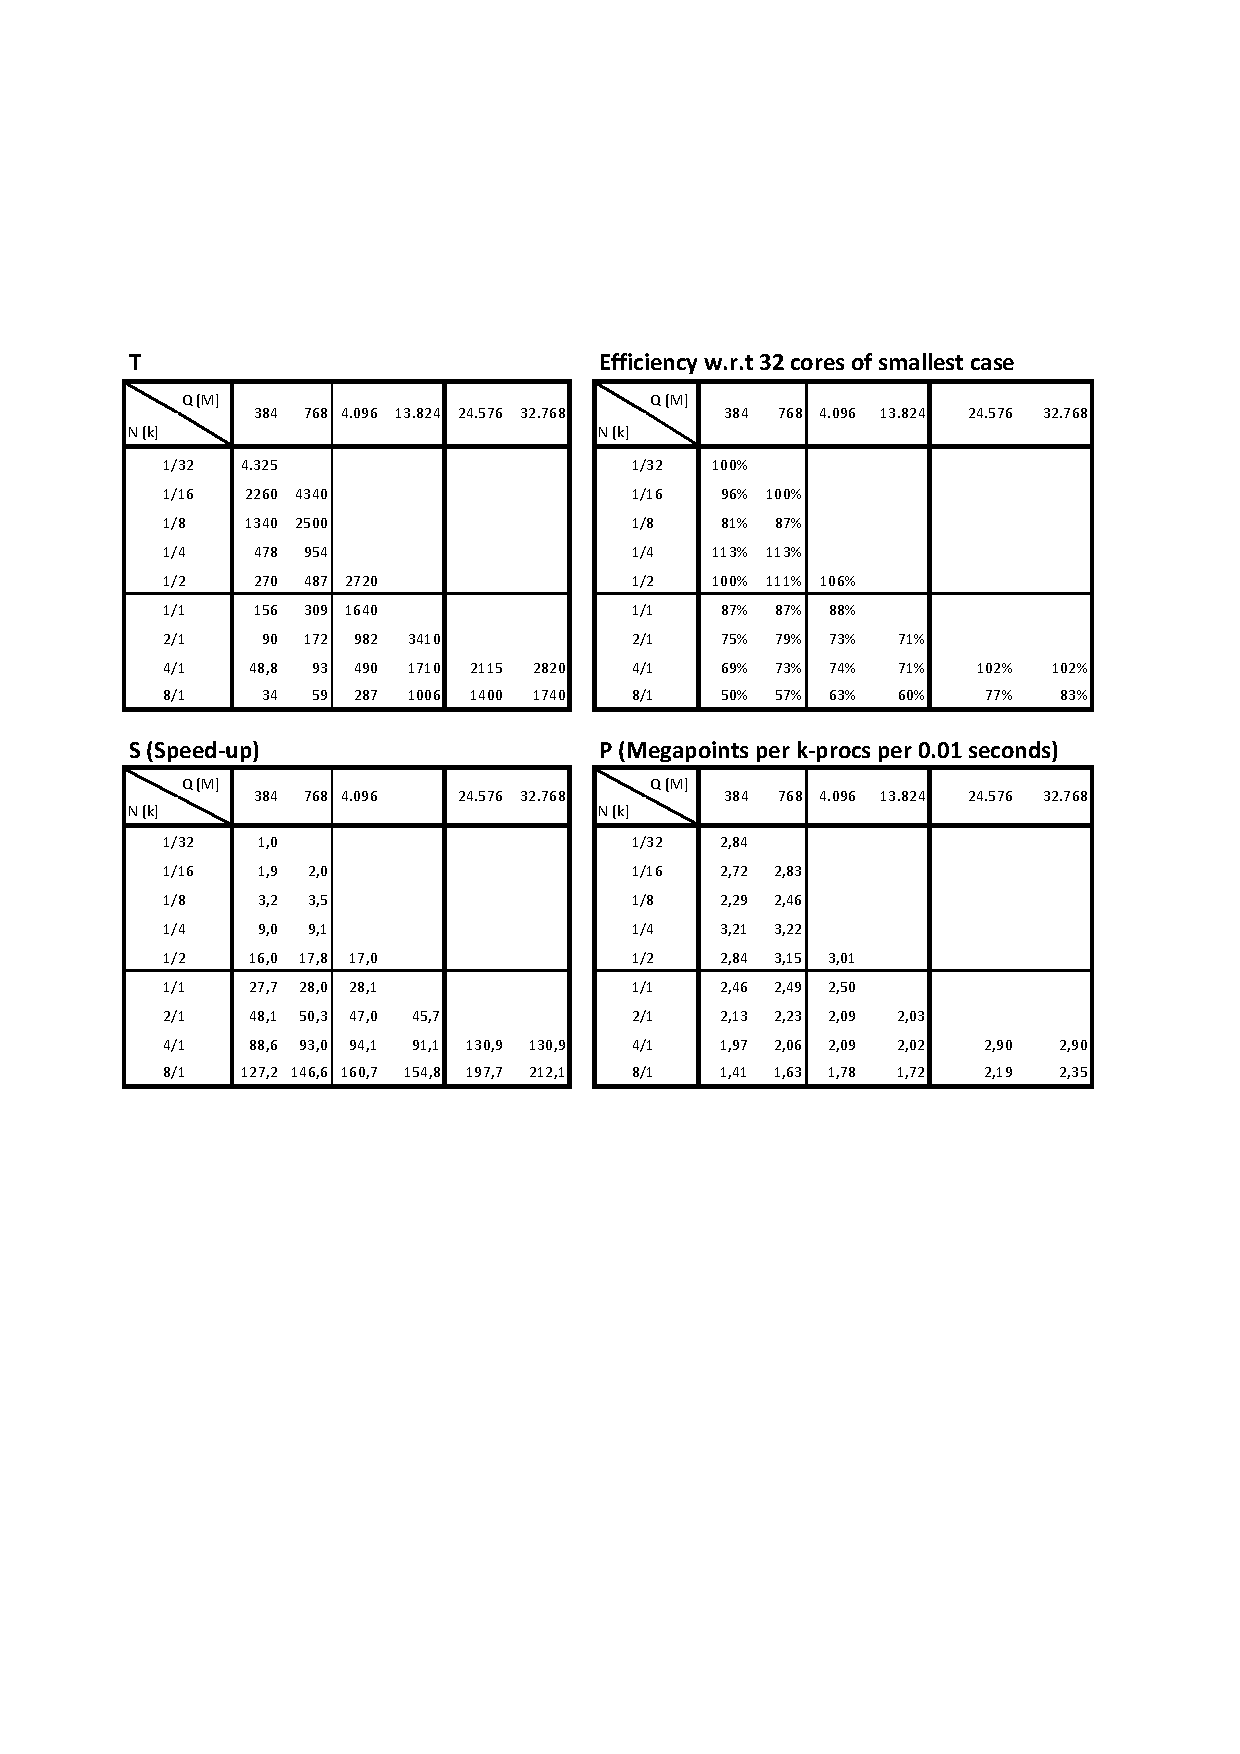
\includegraphics[width=1.0\textwidth]{figs/scaling_overview.pdf}
\end{centering}
\caption{Scaling results in term of Speed-Up $S_W$, Efficiency $E_W$ and
Performance $P$ as defined above.}
\label{fig:v_scaling1}
\end{figure}

The scaling as described in the above paragraph is summarized in the tables
shown in Figure \ref{fig:v_scaling1}. The first table contains the real time
needed for one Runge-Kutta stage, measure in hundredths of a second. As already
said before, these data is simply collected from the matrices on
Figures \ref{fig:matrices1} and \ref{fig:matrices2}. The other 3 tables in
Figure \ref{fig:v_scaling1} contain the corresponding values of $P$, $\eta_v$
and $S_v$.  Figure \ref{fig:v_scaling2} shows the speed-up $S_v$. In the upper
panel there is one line for each cases.  Note, that the definition of $S_v$
does \textbf{not imply that cases start on the linear scaling line}. In this
case, it is part of the measurements and simply means that $\eta_v\approx 100\%$
or $P\approx P_\mathrm{ref}$.

\begin{figure}
  \begin{centering}
  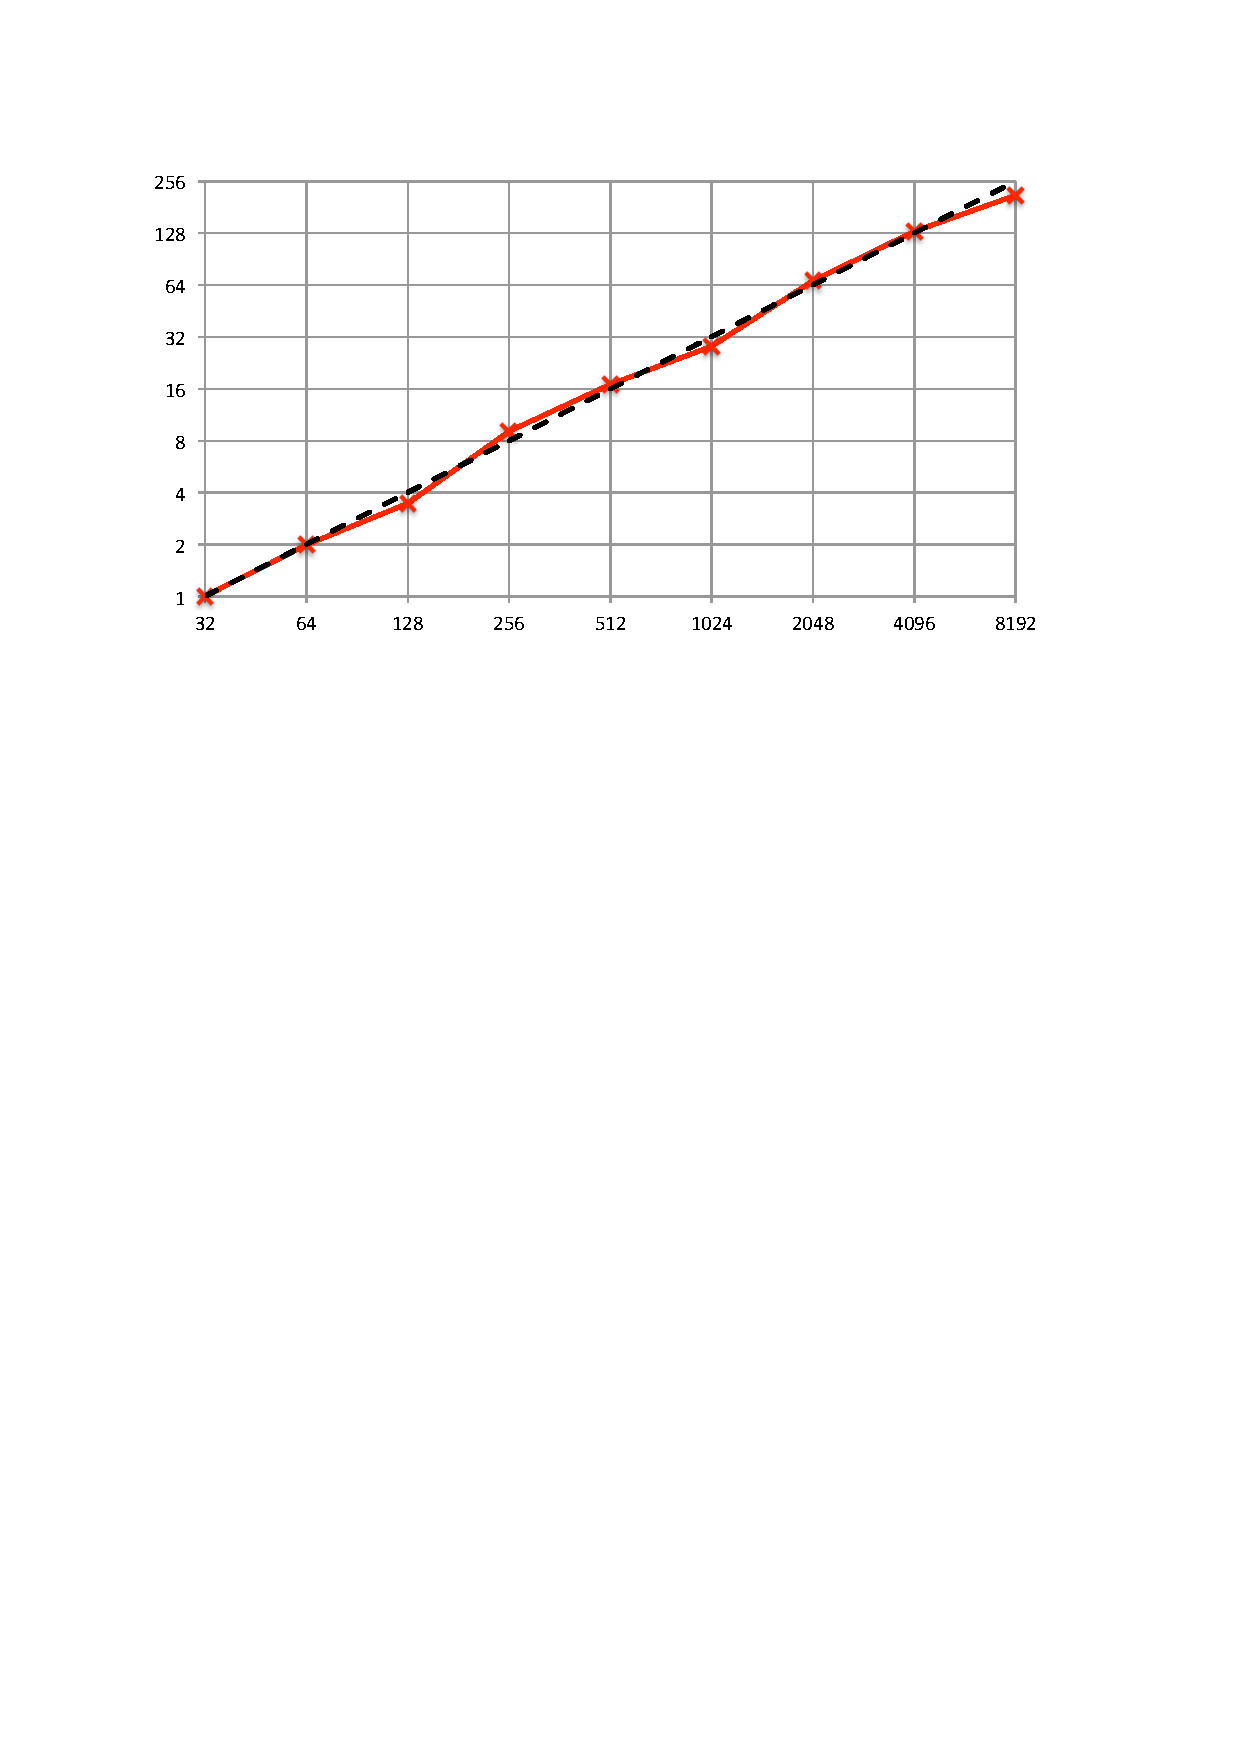
\includegraphics[width=0.5\textwidth]{figs/weak_scaling1.pdf}%
  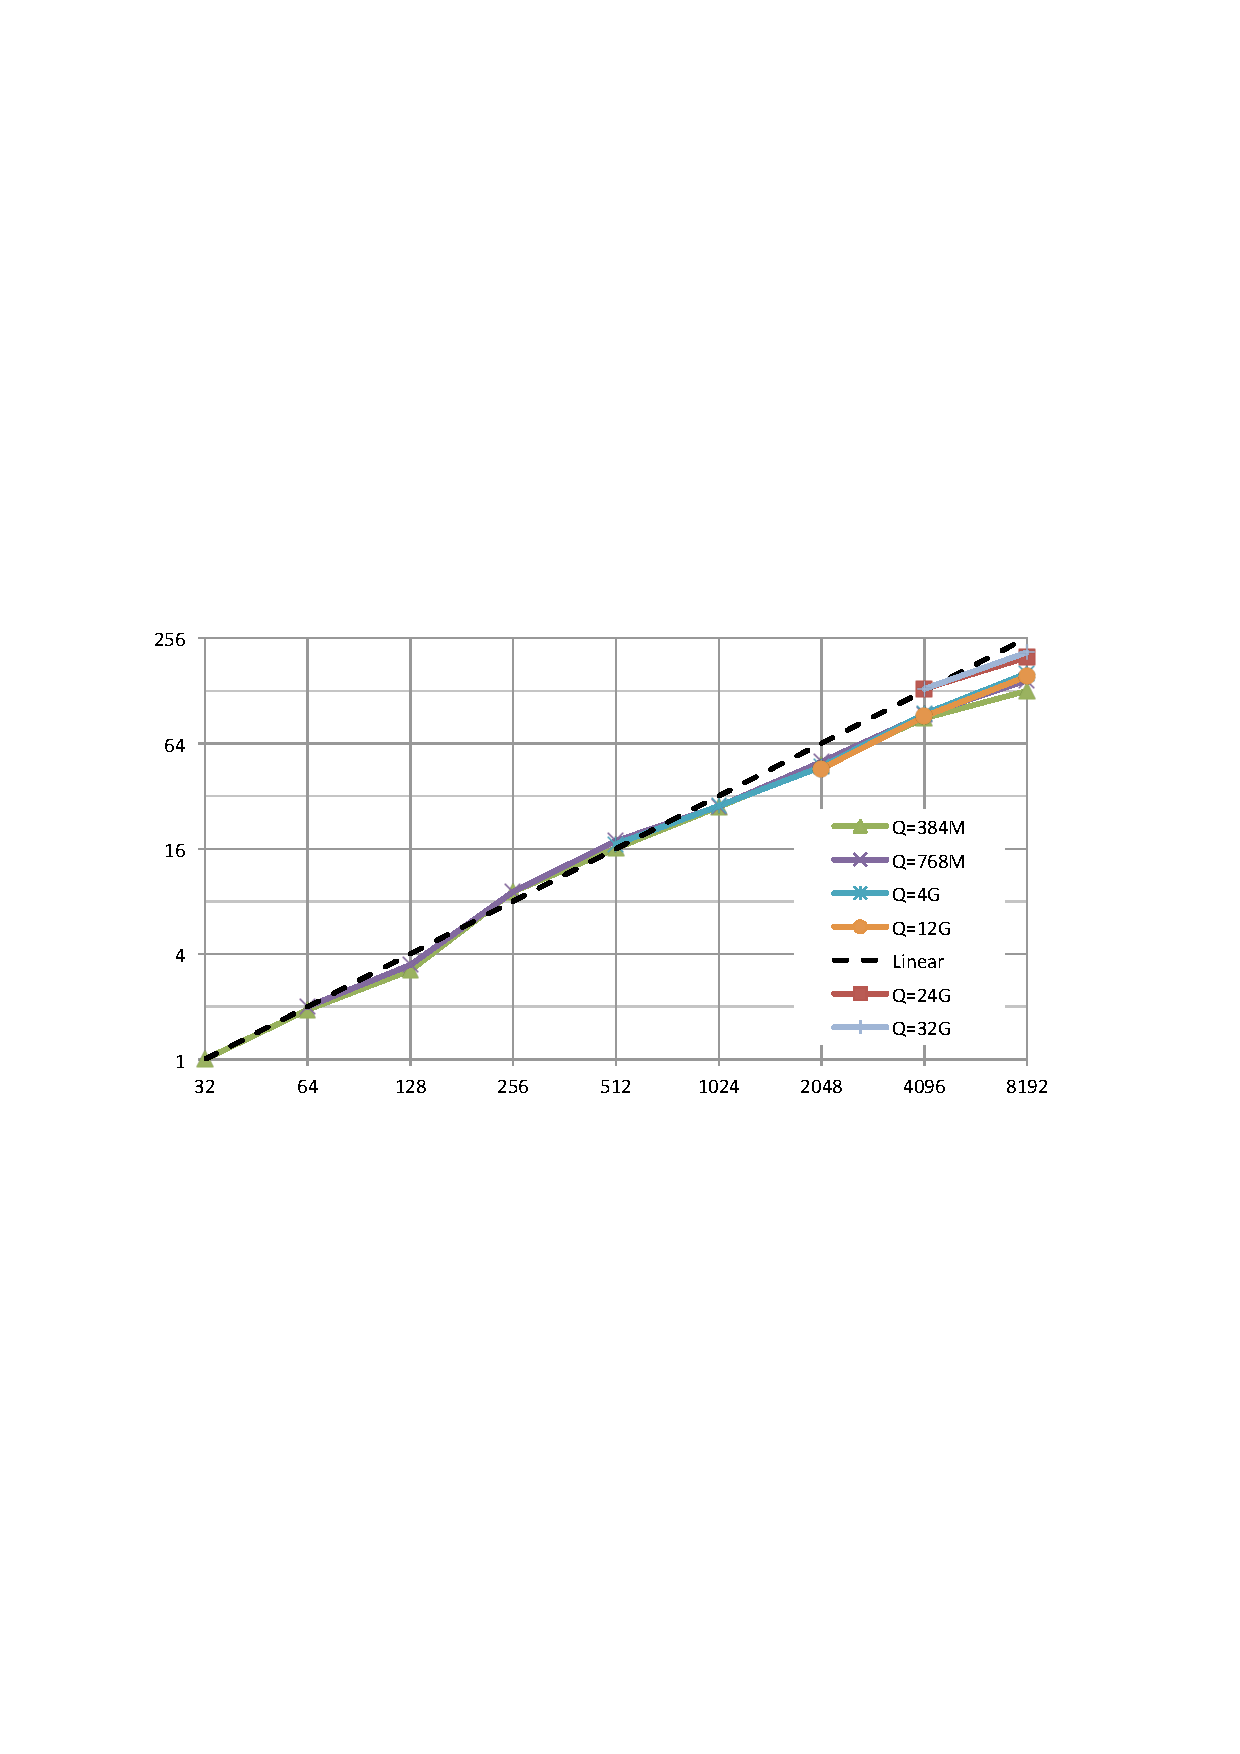
\includegraphics[width=0.5\textwidth]{figs/weak_scaling2.pdf}\\
  \end{centering}
  \caption{Upper panel: $S_W$ versus number of nodes for all geometries. Lower
    panel: maximum speedup for a given number of processors $\max(S_W)|_N$; axes
    as in upper panel.  }
  \label{fig:v_scaling2}
\end{figure}


\section{Scaling on the cluster \texttt{juwels@fz-juelich.de}}

With two sockets each holding 24 CPU cores, juwels features 48 physical cores per node and thus
introduces a single prime factor three to the number CPUs available. To optimally utilize this,
domain sizes should also contain a prime factor three.

The cluster is heterogeneous and features
\begin{itemize}
  \item[(1)] a partition \texttt{batch} with 2271 standard-memory nodes (2x24 cores, 96 GB )
  \item[(2)] a partition \texttt{mem192} with 240 enhanced-memory nodes (2x24 cores, 192 GB )
  \item[(3)] a booster module with 56 GPU-accelerated nodes ( 2x20 cores + 4 GPUs, 192 GB; to be extended in 2020).
\end{itemize}

Scaling was tested using up to 512 nodes on the \texttt{batch} partition (Tab.~\ref{tab:scaling_juwels} and Fig.~\ref{fig:scaling_juwels}
and up to 64 nodes of the \texttt{mem192} partition (Tab.~\ref{tab:memory_juwels}).
There appears to be a significnat memory-overhead of the underlying MPI
which sometimes enables to run particular cases in much less than half the number of large-memory nodes as compared
to running the same configuration in the \texttt{batch partition}.

In comparison with juwels, the normaliezd performance (CPU-h per $1024^3$ points per iteration) is better by up to a factor of $3$, but only for relatively small cases that can be run within a few (up to 4) nodes. For operational cases (using 32 to 128 nodes), the performance boost is around $2$. For even larger cases utilizing 256 or more nodes, performance boost in comparison with juwels is smaller than 2, and it approaches one from above for jobs using 10000 or more MPI tasks.
%
\begin{table}
  \caption{Scaling of two cubed cases in the batch partition of \texttt{juwels@fz-juelich.de}; only computation no initialization, no I/O}
  {\footnotesize\begin{tabular}{r | r r r | r r r | rrr}
    \toprule
    Case   & \multicolumn{3}{c|}{$1536^3$} & \multicolumn{3}{c}{$3072^3$}\\
    \midrule
    \#nodes&        time/it $[s]$ & Speed-up & Eff. & Time/it $[s]$ & Speed-up & Eff.\\
    \midrule
                        8 &      113.5&   1.0&  1.00 \\
    \rowcolor{gray!20} 16&        57.5&   2.0&  0.99\\
                       32&        36.3&   3.1&  0.78\\
    \rowcolor{gray!20} 64&        21.2&   5.4&  0.67& 163.0& 1.0& 1.00\\
                       96&        15.1&   7.5&  0.63&  98.4& 1.7& 1.10\\
    \rowcolor{gray!20}128&        11.5&   9.9&  0.62&  92.8& 1.8& 0.88\\
                      192&         9.1&  12.5&  0.52&  65.1& 2.5& 0.83\\
    \rowcolor{gray!20}256&         6.7&  16.9&  0.53&  51.4& 3.2& 0.79\\
                      384&                        &&&  38.1& 4.3& 0.71\\
    \rowcolor{gray!20}512&                        &&&  29.3& 5.6& 0.70\\
    \bottomrule
  \end{tabular}}
  \label{tab:scaling_juwels}
\end{table}

\begin{table}
  \caption{Average timing for total production jobs in the large-memory partition as compared to the batch partition.
  The batch case using 128 nodes is the smallest configuration for which the case runs in the batch queue. }
  \begin{centering}{\footnotesize\begin{tabular}{rrr|r|rrr}
    \toprule
    Partition               && \multicolumn{4}{c}{mem192}&batch\\
    \#nodes                 &[1]&    20  &  24  &  32 &  64 & 128\\
    \midrule
    \rowcolor{gray!20}\#tasks per node        &[1]&    16  &  48  &  48 &  48 &  48\\
    Wall-clock time/it &[s]      &    422 &  286 & 230 & 115 & 76 \\
    \rowcolor{gray!20} Memory used / node& [GB] &    187 &  160 & 124 &  81 & 52 \\
    total memory & [TB]       &    3.65&  3.75& 3.88& 5.06& 6.5\\
    \rowcolor{gray!20}node-h / it & [h]             &    2.34& 1.91 & 2.04& 2.05& 2.70\\
    \midrule
    Speed-up w.r.t. batch & $[$\%$]$  &    11& \cellcolor{green!62}{\textbf{31}}&22&22&  -\\
    \midrule\bottomrule

  \end{tabular}}\\\end{centering}
  \label{tab:memory_juwels}
\end{table}


\begin{figure}
  % \centering\includegraphics[width=0.66\textwidth]{figs/strong_scaling_juwels.pdf}
  MISSING FIGURE
  \caption{Strong scaling on juwels (solid lines); dashed lines indicated weak scaling.}
  \label{fig:scaling_juwels}
\end{figure}

\section{Scaling on the cluster \texttt{blizzard@dkrz.de}}

To be done.
